% This tex file is available under a
% Creative Commons Attribution-Share Alike license (CC BY-SA 2.0).
% http://creativecommons.org/licenses/by-sa/2.0/
% Copyright © 2013 Rodrigo Hausen
\documentclass{beamer}
\usepackage[utf8]{inputenc}
\usepackage{lmodern}
\usepackage[T1]{fontenc}
\usepackage[portuguese,brazil]{babel}
\usepackage{url}
\usepackage{listings}
\usepackage{color}
\usepackage{textcomp}
\usepackage{pdfpages}
\usepackage{fancyvrb}
\usepackage{enumerate}
\usepackage{icomma} % para vírgula decimal / decimal comma
\definecolor{listinggray}{gray}{0.9}
\definecolor{lbcolor}{rgb}{0.9,0.9,0.9}
\lstset{
    backgroundcolor=\color{lbcolor},
    tabsize=4,
    rulecolor=,
    basicstyle=\scriptsize,
    upquote=true,
    aboveskip={1.5\baselineskip},
    columns=fixed,
    showstringspaces=false,
    extendedchars=true,
    breaklines=true,
    prebreak = \raisebox{0ex}[0ex][0ex]{\ensuremath{\hookleftarrow}},
    frame=single,
    showtabs=false,
    showspaces=false,
    showstringspaces=false,
    identifierstyle=\ttfamily,
    keywordstyle=\color[rgb]{0,0,1},
    commentstyle=\color[rgb]{0.133,0.545,0.133},
    stringstyle=\color[rgb]{0.627,0.126,0.941},
}

\definecolor{pinegreen}{RGB}{0,139,114}
\newcommand{\comment}[1]{{\color{structure.fg!70!white}\footnotesize #1}}

\def\A{\texttt{A}}
\def\B{\texttt{B}}
\def\C{\texttt{C}}
\def\D{\texttt{D}}
\def\E{\texttt{E}}
\def\F{\texttt{F}}

\usetheme{Boadilla}
%\usetheme{umbc2}
\usefonttheme{structuresmallcapsserif}
\usecolortheme{seahorse}

\title{Aula 2: Conversão entre Bases, Aritmética}
\subtitle{Circuitos Digitais}
\author{Rodrigo Hausen}
\institute{CMCC -- UFABC} 
\date{25 de janeiro de 2013}

\begin{document}

\begin{frame}
\maketitle

\vspace{-1cm}

\begin{center}
\url{http://compscinet.org/circuitos}
\end{center}

\end{frame}

%%%%%%%%%%%%%%%%%%%%%%%%%%%%%%%%%%%%%%%%%%%%

\begin{frame}
\frametitle{conversão da base $10$ para base $d$}

números positivos menores do que $1$: $(0,a_{-1} a_{-2} \ldots)_{10}$ para base $2$

Ex1.: $(0,8125)_{10}$ p/ base $2$

\pause

\vspace{12pt}

Grande sacada: observe que $(0,a_{-1} a_{-2} a_{-3} \ldots)_d \times d = (a_{-1}, a_{-2} a_{-3} \ldots)_d$

\pause

\begin{eqnarray*}
(0,8125)_{10} \times 2 & = & (\fbox{1},6250)_{10} \hspace{2cm} a_{-1} = 1\\
\pause
(0,6250)_{10} \times 2 & = & (\fbox{1},25)_{10} \hspace{2cm} a_{-2} = 1\\
\pause
(0,25)_{10} \times 2 & = & (\fbox{0},50)_{10} \hspace{2cm} a_{-3} = 0\\
\pause
(0,50)_{10} \times 2 & = & (\fbox{1},0)_{10} \hspace{2cm} a_{-4} = 1\\
\pause
(0,0)_{10} \times 2 & = & (\fbox{0},0)_{10} \hspace{2cm} a_{-5} = 0\\
\vdots & \vdots & \vdots
\end{eqnarray*}

$(0,8125)_{10} = (0,1101)_2$
\end{frame}

%%%%%%%%%%%%%%%%%%%%%%%%%%%%%%%%%%%%%%%%%%%%

\begin{frame}
\frametitle{conversão da base $10$ para base $d$}

Ex2.: $(0,1)_{10}$ para base $2$ \comment{(na lousa)}

\vspace{12pt}
\pause

$(0,1)_{10} = (0,0\overline{0011}\ldots)_2$

\vspace{12pt}
\pause

CUIDADO! Nem todo número fracionário que possui representação finita na base $10$, também possui representação finita em outras bases.

\vspace{12pt}
\pause

Ex3.: $(6,22)_{10}$ para base $2$

\pause
$110,0\overline{01110000101000111101}\ldots$

\vspace{12pt}

Ex3.: $(6,22)_{10}$ para base $16$

\pause
$6,3\overline{851EB}\ldots$

\end{frame}

\begin{frame}
\frametitle{conversão da base $2$ para base $16$ e vice-versa} 

\begin{itemize}
\item Tabela de conversão entre números de um dígito em base $16$ para números de $4$ dígitos na base $2$\\
\begin{minipage}{0.6\textwidth}
\begin{tabular}{cc r cc}
Base $16$ & Base $2$ & & Base $16$ & Base $2$ \\
\cline{1-2}\cline{4-5}
$0$       & $0000$   & & $8$       & $1000$  \\
\cline{1-2}\cline{4-5}
$1$       & $0001$   & & $9$       & $1001$ \\
\cline{1-2}\cline{4-5}
$2$       & $0010$   & & $\A{}$    & $1010$ \\
\cline{1-2}\cline{4-5}
$3$       & $0011$   & & $\B{}$    & $1011$ \\
\cline{1-2}\cline{4-5}
$4$       & $0100$   & & $\C{}$    & $1100$ \\
\cline{1-2}\cline{4-5}
$5$       & $0101$   & & $\D{}$    & $1101$ \\
\cline{1-2}\cline{4-5}
$6$       & $0110$   & & $\E{}$    & $1110$ \\
\cline{1-2}\cline{4-5}
$7$       & $0111$   & & $\F{}$    & $1111$
\end{tabular}
\end{minipage}
\pause
\begin{minipage}{0.32\textwidth}
Todos os inteiros de até $4$ dígitos em base $2$ correspondem a números de exatamente $1$ dígito em base $16$
\end{minipage}

\item Ex1.: $({\color{red}\C{}}{\color{blue}5},{\color{pinegreen}3}\E{})_{16} = ( \uncover<3->{{\color{red}1100}}\uncover<4->{{\color{blue}0101},}\uncover<5->{{\color{pinegreen}0011}\uncover<6->{1110}} )_2$
\uncover<7->{
    \item Ex2.: $(\only<7-8>{\uncover<8->{000}10010,1001010\uncover<8->{0}}\only<9>{{\color{red}0001}{\color{blue}0010},{\color{pinegreen}1001}0100})_2 = ( \uncover<9>{{\color{red}1}{\color{blue}2},{\color{pinegreen}9}4} )_{16}$
}
\end{itemize}

\end{frame}

\begin{frame}
\frametitle{Conversão base $16$ para base $2$ e vice-versa}

\begin{itemize}
\item \textbf{De 16 para 2}: substitua cada dígito na base $16$ pelos $4$ dígitos correspondentes na base $2$
\[
    ({\color{red}\C{}}{\color{blue}5},{\color{pinegreen}3}\E{})_{16} = ( {{\color{red}1100}}{{\color{blue}0101},}{{\color{pinegreen}0011}{1110}} )_2
\]\\[-12pt]
\pause
\item \textbf{De 2 para 16}: agrupe de $4$ em $4$ os dígitos a partir da vírgula (da vírgula para os extremos). Considere como zeros os dígitos que estejam faltando para completar algum grupo.
\[
    ({\color{red}11}{\color{blue}1110},{\color{pinegreen}1001}101)_2 = ( {\color{red}3}{\color{blue}\E},{\color{pinegreen}9}\A{} )_{16}
\]\\[-12pt]
\pause
\item Também é fácil converter da base $2$ para a base $8$ e vice-versa.\\
$(73,44)_8 = (111011,100100)_2$ e
$(11{\color{blue}001}{\color{pinegreen}011}{\color{red}101},
{\color{blue}110}{\color{pinegreen}110}{\color{red}1})_2 =
(3{\color{blue}1}{\color{pinegreen}3}{\color{red}5},{\color{blue}6}{\color{
pinegreen}6}{\color{red}4})_8$\\
(note que todos os inteiros com até $3$ algarismos na base $2$ podem ser representados por apenas $1$ algarismo na base $8$) 
\end{itemize}

\end{frame}

\begin{frame}
\frametitle{Bases mais utilizadas em computação}

\begin{itemize}
\item Por razões que veremos mais à frente, a base $2$ é a base mais usada em
computação hoje em dia.
\pause
\item Note que um número inteiro costuma ter menos dígitos quando é representado
numa base maior.
\[
    (1111110)_2 = (126)_{10} = (7\E)_{16}
\]\\[-12pt]
\pause
\item Como é muito fácil converter da base $2$ para as bases $8$ e $16$ e
vice-versa, estas bases costumam também ser muito usadas.
\pause
\item \textbf{Para casa}:
\begin{enumerate}
  \item um número inteiro com exatamente $n$ dígitos quando representado na base
$2$ terá, no mínimo, quantos dígitos em sua representação decimal?
  \item e no máximo? 
  \item dado um número inteiro cuja representação decimal
possui $N$ dígitos, quantos dígitos serão necessários, no máximo, para
representá-lo na base $2$?
\end{enumerate}
\end{itemize}
\end{frame}

\begin{frame}
\frametitle{Bases mais utilizadas em computação}

Nomes para as bases mais usadas:

\begin{itemize}
  \item Base $2$ = base binária
  \item Base $8$ = base octal
  \item Base $10$ = base decimal
  \item Base $16$ = base hexadecimal
\end{itemize}

Além dessas, há outras bases menos usadas em computação, tais como a base $64$,
que não possuem nomes especiais.
\end{frame}

\begin{frame}
\frametitle{Aritmética}

Perguntas que responderemos hoje:

\begin{itemize}
\item Por que quando somamos dois números na base $10$, podemos colocar ``um
sobre o outro'' e somar os dígitos individualmente, tomando cuidado com o ``vai
um''?
\item Qual o significado do ``vai um''?
\item Será que o mesmo procedimento de soma também funciona em outras bases?
\end{itemize}
\end{frame}

\begin{frame}
\frametitle{Analisando a soma}

Ex.: $397 + 654 = 1051$\\[4pt]

\begin{center}
\begin{tabular}{c@{\,}c@{\,}c@{\,}cl}
 1 & 1 & 1 &   & $\leftarrow$ ``vai-uns''\\
   & 3 & 9 & 7 &   \\
   & 6 & 5 & 4 & + \\
\cline{1-4}
 1 & 0 & 5 & 1
\end{tabular}
\end{center}\vspace{-8pt}
\pause
\begin{eqnarray*}
397 & = & 3\cdot10^2 + 9\cdot10^1 + 7\cdot10^0\\
\pause
+ 654 & = & 6\cdot10^2 + 5\cdot10^1 + 4\cdot10^0\\
\pause
397 + 654 & = & (3+6)\cdot10^2 + (9+5)\cdot10^1 + (7+4)\cdot10^0 \\
\pause
          & = & (3+6)\cdot10^2 + (9+5)\cdot10^1 + (11)\cdot10^0 \\
\pause
          & = & (3+6)\cdot10^2 + (9+5)\cdot10^1 +
\underbrace{1\cdot10^1}_{\text{vai um}} + 1\cdot10^0 \\
\pause
          & = & (3+6)\cdot10^2 + (9+5+1)\cdot10^1 + 1\cdot10^0 \\
\pause
          & \vdots & \vdots \\
    \uncover<9>{1051}  & = & 1\cdot10^3 + 0\cdot10^2 + 5\cdot10^1 + 1\cdot10^0
\end{eqnarray*}

\end{frame}


\begin{frame}
\frametitle{Algoritmo da soma}

\textbf{Entrada}: números com $n$ algarismos $A = a_{n-1} a_{n-2} \ldots a_1
a_0$ e $B = b_{n-1} b_{n-2} \ldots b_1 b_0$\\
\textbf{Saída}: número $C = c_n c_{n-1} c_{n-2} \ldots c_1 c_0$ com $n+1$
algarismos que representa a soma $A+B$.\\[12pt]

\def\ts{\hspace{2ex}}

\begin{minipage}{0.55\textwidth}
\begin{semiverbatim}
VaiUm $\leftarrow$ 0

PARA $i$ = 0\ldots{}n-1

\ts SE VaiUm = 0

\ts\ts  c$_i$ $\leftarrow$ Tabuada[a$_i$][b$_i$]

\ts\ts VaiUm $\leftarrow$ TemVaiUm[a$_i$][b$_i$]

\ts SENÃO

\ts\ts  c$_i$ $\leftarrow$ TabuadaComVaiUm[a$_i$][b$_i$]

\ts\ts VaiUm $\leftarrow$ VaiUmComVemUm[a$_i$][b$_i$]
\vspace{-12pt}
c$_n$ $\leftarrow$ VaiUm
\end{semiverbatim}
\end{minipage}%
\only<2>{%
\begin{minipage}{0.41\textwidth}%
{\scriptsize{Tabuada = Matriz[10][10]}}
\resizebox{0.99\textwidth}{!}{
\begin{tabular}{c|cccccccccc}
  & 0 & 1 & 2 & 3 & 4 & 5 & 6 & 7 & 8 & 9 \\
\hline
0 & 0 & 1 & 2 & 3 & 4 & 5 & 6 & 7 & 8 & 9 \\
1 & 1 & 2 & 3 & 4 & 5 & 6 & 7 & 8 & 9 & 0 \\
2 & 2 & 3 & 4 & 5 & 6 & 7 & 8 & 9 & 0 & 1 \\
3 & 3 & 4 & 5 & 6 & 7 & 8 & 9 & 0 & 1 & 2 \\
\vdots & \vdots & \vdots & \vdots & \vdots & \vdots &\vdots & \vdots & \vdots
&\vdots & \vdots\\
9 & 9 & 0 & 1 & 2 & 3 & 4 & 5 & 6 & 7 & 8
\end{tabular}%
}%
\end{minipage}
}%
\only<4>{%
\begin{minipage}{0.41\textwidth}
{\scriptsize{TemVaiUm = Matriz[10][10]}}
\resizebox{0.99\textwidth}{!}{
\begin{tabular}{c|cccccccccc}
  & 0 & 1 & 2 & 3 & 4 & 5 & 6 & 7 & 8 & 9 \\
\hline
0 & 0 & 0 & 0 & 0 & 0 & 0 & 0 & 0 & 0 & 0 \\
1 & 0 & 0 & 0 & 0 & 0 & 0 & 0 & 0 & 0 & 1 \\
2 & 0 & 0 & 0 & 0 & 0 & 0 & 0 & 0 & 1 & 1 \\
3 & 0 & 0 & 0 & 0 & 0 & 0 & 0 & 1 & 1 & 1 \\
\vdots & \vdots & \vdots & \vdots & \vdots & \vdots &\vdots & \vdots & \vdots
&\vdots & \vdots\\
9 & 0 & 1 & 1 & 1 & 1 & 1 & 1 & 1 & 1 & 1
\end{tabular}
}%
\end{minipage}%
}%
\only<3>{%
\begin{minipage}{0.41\textwidth}
{\scriptsize{TabuadaComVaiUm = Matriz[10][10]}}
\resizebox{0.99\textwidth}{!}{
\begin{tabular}{c|cccccccccc}
  & 0 & 1 & 2 & 3 & 4 & 5 & 6 & 7 & 8 & 9 \\
\hline
0 & 1 & 2 & 3 & 4 & 5 & 6 & 7 & 8 & 9 & 0 \\
1 & 2 & 3 & 4 & 5 & 6 & 7 & 8 & 9 & 0 & 1 \\
2 & 3 & 4 & 5 & 6 & 7 & 8 & 9 & 0 & 1 & 2 \\
3 & 4 & 5 & 6 & 7 & 8 & 9 & 0 & 1 & 2 & 3 \\
\vdots & \vdots & \vdots & \vdots & \vdots & \vdots &\vdots & \vdots & \vdots
&\vdots & \vdots\\
9 & 0 & 1 & 2 & 3 & 4 & 5 & 6 & 7 & 8 & 9
\end{tabular}%
}%
\end{minipage}%
}%
\only<5>{%
\begin{minipage}{0.41\textwidth}
{\scriptsize{VaiUmComVemUm = Matriz[10][10]}}
\resizebox{0.99\textwidth}{!}{
\begin{tabular}{c|cccccccccc}
  & 0 & 1 & 2 & 3 & 4 & 5 & 6 & 7 & 8 & 9 \\
\hline
0 & 0 & 0 & 0 & 0 & 0 & 0 & 0 & 0 & 0 & 1 \\
1 & 0 & 0 & 0 & 0 & 0 & 0 & 0 & 0 & 1 & 1 \\
2 & 0 & 0 & 0 & 0 & 0 & 0 & 0 & 1 & 1 & 1 \\
3 & 0 & 0 & 0 & 0 & 0 & 0 & 1 & 1 & 1 & 1 \\
\vdots & \vdots & \vdots & \vdots & \vdots & \vdots &\vdots & \vdots & \vdots
&\vdots & \vdots\\
9 & 1 & 1 & 1 & 1 & 1 & 1 & 1 & 1 & 1 & 1
\end{tabular}
}%
\end{minipage}%
}%
\end{frame}

\begin{frame}
\frametitle{Algoritmo da soma}

\begin{itemize}
 \item Como somar números em outra base, p. ex., 2?
\end{itemize}

Ex.: $(101011)_2 + (100111)_2 = (1010010)_2$, ou seja, $(43)_{10} + (39)_{10}
= (82)_{10}$\\[4pt]

\begin{center}
\begin{tabular}{c@{\,}c@{\,}c@{\,}c@{\,}c@{\,}c@{\,}cl}
 1 &   & 1 & 1 & 1 & 1 &   & $\leftarrow$ ``vai-uns''\\
   & 1 & 0 & 1 & 0 & 1 & 1 & \\
   & 1 & 0 & 0 & 1 & 1 & 1 & + \\
\cline{1-7}
 1 & 0 & 1 & 0 & 0 & 1 & 0 &
\end{tabular}
\end{center}

\pause

Tabuada na base $2$: bem mais simples!\\[6pt]

\pause

\begin{minipage}{0.19\textwidth}
Tabuada

\begin{tabular}{c|cc}
   & 0 & 1 \\
\hline
 0 & 0 & 1 \\
 1 & 1 & 0
\end{tabular}
\end{minipage}
\begin{minipage}{0.19\textwidth}
TemVaiUm

\begin{tabular}{c|cc}
   & 0 & 1 \\
\hline
 0 & 0 & 0 \\
 1 & 0 & 1
\end{tabular}
\end{minipage}
\begin{minipage}{0.29\textwidth}
TabuadaComVaiUm

\begin{tabular}{c|cc}
   & 0 & 1 \\
\hline
 0 & 1 & 0 \\
 1 & 0 & 1
\end{tabular}
\end{minipage}
\begin{minipage}{0.29\textwidth}
VaiUmComVemUm

\begin{tabular}{c|cc}
   & 0 & 1 \\
\hline
 0 & 0 & 1 \\
 1 & 1 & 1
\end{tabular}
\end{minipage}

\end{frame}

\begin{frame}
\frametitle{Subtração binária}

\begin{itemize}
\item $A - B = C$, $A$ é o minuendo, $B$ é o subtraendo
\item Da direita para a esquerda, algarismo por algarismo
\item Se o algarismo do minuendo é menor que o do subtraendo, ``empresta'' do algarismo à esquerda
\end{itemize}

Ex.: $110001 - 10011$\\[6pt]

\only<1>{\includegraphics{images/subtracao_1}}%
\only<2>{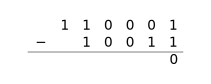
\includegraphics{images/subtracao_2}}%
\only<3>{\includegraphics{images/subtracao_3}}%
\only<4>{\includegraphics{images/subtracao_4}}%
\only<5>{\includegraphics{images/subtracao_5}}%
\only<6>{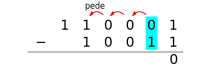
\includegraphics{images/subtracao_6}}%
\only<7>{\includegraphics{images/subtracao_8}}%
\only<8>{\includegraphics{images/subtracao_9}}%
\only<9>{\includegraphics{images/subtracao_10}}%
\only<10>{\includegraphics{images/subtracao_11}}%
\only<11>{\includegraphics{images/subtracao_12}}%
\only<12>{\includegraphics{images/subtracao_13}}%
\only<13>{\includegraphics{images/subtracao_14}}%
\only<14>{\includegraphics{images/subtracao_15}}%
\only<15>{\includegraphics{images/subtracao_16}}%
\only<16>{\includegraphics{images/subtracao_17}}%
\only<17>{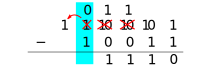
\includegraphics{images/subtracao_19}}%
\only<18>{\includegraphics{images/subtracao_20}}%
\only<19>{\includegraphics{images/subtracao_21}}%
\only<20>{\includegraphics{images/subtracao_23}}%
\only<21->{\includegraphics{images/subtracao_24}}%

\uncover<22>{$= 11110$}
\end{frame}

\begin{frame}
\frametitle{Subtração binária}

\begin{itemize}
\item Jeito fácil: usando complemento a $2$
\end{itemize}

Ex.: $110001 - 10011$

\pause

\begin{itemize}
\item Complemento a $1$ de $10011$ com $6$ algarismos (maior quantidade de algarismos entre minuendo e subtraendo):
$$\underbrace{111111}_{6 \text{ uns}} - 10011 = 101100$$
\pause
\vspace{-12pt}
\item Complemento a $1$ de número binário: troca $1$ por $0$ e vice-versa
\pause
\item Complemento a $2$: é o complemento a $1$, adicionado de $1$ unidade:
$$111111 - 10011 {\color{red}+ 1} = 101101$$
\pause
\vspace{-12pt}
\item Denotaremos o complemento a $2$ de um número $B$ por $$\overline{B} + 1$$
\vspace{-12pt}
\end{itemize}

\end{frame}

\begin{frame}
\frametitle{Subtração binária}

Usando complemento a $2$:

\begin{itemize}
\item $A - B = A + (\overline{B} + 1)$, desprezando o último ``vai-um''
\end{itemize}

Ex.: $110001 - 10011$\\[12pt]

$A = 110001$, $B = 10011$\\[12pt]

\pause

$\overline{B} = 101100$\pause, $\overline{B} + 1 = 101101$\\[12pt]

\pause

\def\cutout{\hspace{-1.2ex}{\color{red}\textbf{/}}\hspace{-1ex}{\color{red}\textbf{\textbackslash}}}

$A + (\overline{B} + 1) =$\\
\begin{tabular}{ccccccccl}
    & 1         &   &   &   &   & 1 &   & vai-uns \\
    &           & 1 & 1 & 0 & 0 & 0 & 1 \\
$+$ &           & 1 & 0 & 1 & 1 & 0 & 1 \\
\hline
    & 1\cutout  & 0 & 1 & 1 & 1 & 1 & 0 \\
\end{tabular}

\end{frame}

\begin{frame}[fragile]
\frametitle{Algoritmo da subtração}

\begin{Verbatim}[commandchars=\\\{\},codes={\catcode`$=3\catcode`^=7}]
Subtração(A[0...n-1], B[0...n-1])
    $\overline{\texttt{B}}$ $\leftarrow$ ComplementoAUm(B)
    Um $\leftarrow$ Array[0...n]
    Um[0] $\leftarrow$ 1
    ComplementoADois $\leftarrow$ Soma($\overline{\texttt{B}}$,Um)
    // descarta n+1-ésimo dígito criado para a soma
    ComplementoADois $\leftarrow$ ComplementoADois[0...n-1]
    C $\leftarrow$ Soma(A, ComplementoADois)
    C $\leftarrow$ C[0...n-1] // descarta vai-um
    RETORNE C \pause
ComplementoAUm(B[0...n-1])
    $\overline{\texttt{B}}$ $\leftarrow$ Array[0...n-1]
    PARA i = 0...n-1 FAÇA
        SE B[i] = 0 ENTÃO $\overline{\texttt{B}}$[i] $\leftarrow$ 1
        SE B[i] = 1 ENTÃO $\overline{\texttt{B}}$[i] $\leftarrow$ 0
    RETORNE $\overline{\texttt{B}}$
\end{Verbatim}

\end{frame}


\begin{frame}
\frametitle{Subtração binária: números negativos}

\begin{itemize}
\item E se o minuendo for menor que o subtraendo? $$A - B < 0 \text{ se } A < B$$
\vspace{-12pt}
\pause
\item O algoritmo tradicional (usando empréstimos) não funciona! Não terá como fazer empréstimo para o algarismo mais à esquerda.
\pause
\item Como efetuar a subtração? Pelo jeito tradicional, é necessário trocar a ordem das parcelas e colocar o sinal de menos à esquerda do resultado.
$$10011 - 110001 = -(110001-10011) = -11110$$ 
\vspace{-12pt}
\pause
\item Note o algoritmo tradicional falha se, e somente se, o minuendo for menor que o subtraendo. E se usarmos complemento a $2$?
\end{itemize}

\end{frame}

\begin{frame}
\frametitle{Subtração binária: números negativos}
Ex.: $10011 - 110001$ usando complemento a $2$.\\[12pt]

$A = 010011$, $B = 110001$\\[12pt]

\pause

$\overline{B} = 001110$, $\overline{B} + 1 = 001111$\\[12pt]

\pause

$A + (\overline{B} + 1) = 010011 + 001111 =$\\[12pt]

\pause

\begin{tabular}{ccccccccl}
    &           & 1 & 1 & 1 & 1 & 1 &   & $\longleftarrow$ vai-uns \\
    &           & 0 & 1 & 0 & 0 & 1 & 1 \\
$+$ &           & 0 & 0 & 1 & 1 & 1 & 1 \\
\hline
    & \fbox{\phantom{1}}  & 1 & 0 & 0 & 0 & 1 & 0 \\
\end{tabular}

\vspace{12pt}

Não tem último vai-um!
\end{frame}

\begin{frame}
\frametitle{Subtração binária: números negativos}

\begin{itemize}
\item Quando estivermos fazendo subtração com complemento a $2$, se não houver o vai-um mais à esquerda -- ou seja, se $c_n$ não for um no algoritmo da soma -- então o minuendo é menor que o subtraendo.
\pause
\item Observe que o resultado da operação, à primeira vista, não faz sentido:\\
$A = 010011$, $B = 110001$\\[6pt]
$A + (\overline{B} + 1) = 010011 + 001111 = 100010 \ne A-B = -11110$
\pause
\item Mas, calculando o complemento a $2$ do resultado:\\
$\overline{100010} + 1 = 011101 + 1 = 011110$ (mágica?)
\end{itemize}

\pause

\begin{minipage}{0.95\textwidth}
\textbf{Para casa}: Para a soma binária, prove que no caso $A = 0 a_{n-2} \ldots a_0$ e $B = 0 b_{n-2} \ldots b_0$, onde $A < B$, então:\\
(1) o resultado da soma $A + (\overline{B} + 1)$ não tem vai-um $c_n$;\\
(2) $\overline{A + (\overline{B} + 1)} + 1 = B - A$.\\
Altere o algoritmo da subtração usando complemento a $2$ para funcionar com diferenças negativas (escreva pseudocódigo).
\end{minipage}

\end{frame}

\begin{frame}
\frametitle{Para casa}

\begin{itemize}
\item Acessar o site \url{http://compscinet.org/circuitos} e ler as informações sobre o curso com cuidado
\pause
\item Obter o livro:\\
Thomas Floyd. Sistemas Digitais: Fundamentos e Aplicações, 9ed. Editora Bookman, 2007.
\pause
\item Leitura recomendada: Floyd, seções 2-1 a 2-6 (menos a parte de números em ponto flutuante), 2-7, 2-8.
\item Exercícios recomendados: autoteste 1 a 16, problemas de 1 a 40 (exceto 27 e 28)
\end{itemize}

\end{frame}

\end{document}
